\chapter{Algoritmi Greedy}
Si tratta di una tecnica che si applica sempre ai problemi di ottimizzazione, ma
rispetto alla programmazione dinamica ha un approccio diverso, dato che il calcolo della
soluzione ottima (in questo caso ne calcola una sola) avviene attraverso una
sequenza di scelte \textbf{localmente} ottime.
\paragraph*{Caratteristiche degli algoritmi Greedy}
\begin{itemize}
    \item Semplici da scrivere
    \item Efficienti
\end{itemize}
\paragraph*{Questioni}
\begin{itemize}
    \item Dimostrare la correttezza di un algoritmo greedy
    \item Capire quali problemi sono affrontabili con una strategia greedy
\end{itemize}
\section{Problema - Selezione attività}
\paragraph*{INPUT} Dato un insieme $A = \{a_1, a_2, \dots, a_n\}$ di n attività, tale
che $a_i = [s_i, e_i)$ per $\ \leq i \leq n$, dove $s_i$ è il tempo di inizio ed $e_i$ è il
tempo di fine.
\begin{center}
    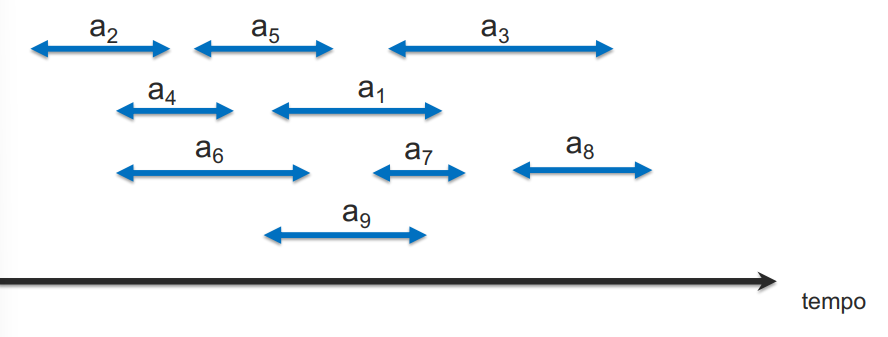
\includegraphics[width=80mm,scale=0.5]{greedy_sel_attivit.png}
\end{center}
$a_i=[s_i, e_i)$ e $a_j = [s_j, e_j)$ sono \textbf{compatibili} se $s_i \geq e_j$ oppure 
$s_j \geq e_i$. In poche parole se un attività inizia nello stesso momento della fine dell'altra, oppure dopo.
Le attività non devono accavallarsi, cioè eseguirsi nello stesso tempo di un'altra.
Facciamo qualche esempio che sicuramente è più semplice.\\
Per esempio $a_5=[s_5, e_5)$ e $a_8 = [s_8, e_8)$ sono compatibili, mentre $a_5 = [s_5, e_5)$ e 
$a_1 = [s_1, e_1)$ NON sono compatibili, infatti l'inizio di $a_1$ è minore della fine di $a_5$.
\paragraph*{OUTPUT} il sottoinsieme X di cardinalità massima composto di attività mutuamente compatibili.
In questo esempio l'OUTPUT desiderato è $X = \{a_2, a_5, a_7, a_8\}$.
\subsection{Soluzione con DP}
$A = \langle a_1, a_2,\dots,a_n\rangle$ tale che $e_1 \leq e_2 \leq \dots \leq e_n$.\\
$A = A \cup \{a_0, a_{n+1}\} = \langle a_0, a_1, \dots, a_n, a_{n+1}\rangle$ tale che $e_0 \leq s_1$
e $s_{n+1} \geq e_n$.
\paragraph*{Sottoproblema (i,j) per $0 \leq i < j \leq n+1$}
Trovare il sottoinsieme $X_{ij}$ di attività mutuamente compatibili di cardinalità massima per
$A_{ij} = \langle a_{i+1}, a_{i+2},\dots,a{j-2}, a{j-1} \rangle$.
\paragraph*{Sottoproblema $(0, n+1)$}
Trovare il sottoinsieme $X_{0,n+1} = X$ di attività mutuamente compatibili di cardinalità
massima per $A_{0,n+1} = \langle a_1, a_2, \dots, a_{n-1}, a_n \rangle = A$.\\
Numero totale di sottoproblemi \ra $(n+1)+n+(n-1)+(n-2)+\dots+1$.
\paragraph*{CASI BASE per $j=i+1 (A_{ij}=\emptyset)$}
$X_{ij} = \emptyset$.
\paragraph*{PASSO RICORSIVO per $j > i +1 (A_{ij} \neq \emptyset)$}
\textbf{Sottostruttura ottima}\\
$a_k$ appartiene a $X_{ij} \implies X_{ij} = X_{ik} \cup \{a_k\} \cup X_{kj}$\\
$X_{ik}$ soluzione ottima di $A_{ik}$\\
$X_{kj}$ soluzione ottima di $A_{kj}$\\
$X_{ij} = max\{X_ik \cup \{a_k\} \cup X_kj \text{ per } i < k < j\}$.
\paragraph*{Valore ottimo - Sostituzione coefficiente all'eqauzione}
\paragraph*{CASI BASE per $j=i+1 (A_{ij}=\emptyset)$}
$c_{ij} = 0$ (valore ottimo)
\paragraph*{PASSO RICORSIVO per $j > i +1 (A_{ij} \neq \emptyset)$}
$c_{ij} = max\{c_{ik} + 1 + c_kj \text{ t.c } i < k < j\}$ (valore ottimo).
\subsection{Svantaggi della Soluzione tramite DP}
\begin{enumerate}
    \item Tutti i sottoproblemi devono essere risolti per arrivare a calcolare il valore ottimo
    \item Si deve in seguito ricostruire la soluzione ottima (soluzione ottimale) perchè io ho solo
    i coefficienti, non ho la sequenza richiesta in OUTPUT
\end{enumerate}
\subsection{Approccio greedy}
\begin{center}
    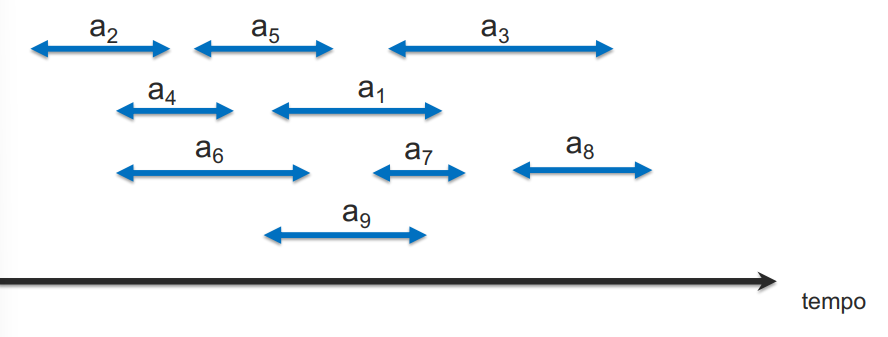
\includegraphics[width=80mm,scale=0.5]{greedy_sel_attivit.png}
\end{center}
In questo caso dobbiamo scegliere un parametro, per esempio \ra Attività con il tempo
di fine più basso, che in questo caso è $a_2$.\\
\textbf{IPOTESI}: $a_2$ appartiene alla soluzione ottima X $\implies X = \{a_2\} \cup X_2$.\\
\textbf{$X_2$ è la soluzione ottima per $A_2 = \{a = [s,e) \in A | \text{ a compatibile con } a_2\}$}
Compatibile con $a_2$ significa che $s \geq e_2$. Graficamente devo avere che la fine di $a_2$ non si
intersechi nessuna attività. Quindi devo cercare l'attività con il tempo di fine più basso in $A_2 \rt a_5$.
\begin{center}
    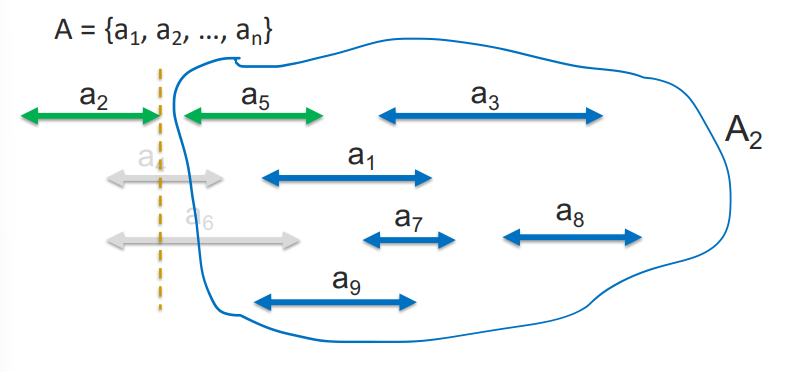
\includegraphics[width=80mm,scale=0.5]{greedy_sel_attivit_p2.png}
\end{center}
Scelgo quindi $a_5$ dato che ha il tempo di fine più basso rispetto a tutte le attività 
compatibili con $a_2$.\\
\textbf{IPOTESI} $a_5$ appartiene alla soluzione ottima $X_2 \implies X = \{a_2\} \cup \{a_5\} \cup X_2$.\\
$X_5$ è soluzione ottima per $A_5 = \{a=[s,e) \in A | s \geq e_5\}$.\\
Ancora una volta cerco le attività compatibili con $a_5$, che abbiano quindi un inizio che sia maggiore
o uguale rispetto alla fine di $a_5$, e scelgo quella con tempo di fine minore.\\
Determino quind che $A_5 \rt a_7$.\\
\textbf{IPOTESI}: $a_7$ appartiene alla soluzione ottima $X_5 \implies X = \{a_2\} \cup \{a_5\} \cup \{a_7\} \cup X_7$.\\
Cerco nuovamente l'attività con tempo di fine più basso rispetto a quelle compatibili con $a_7$ e trovo
che l'attività in questione è $a_8$.\\
\textbf{IPOTESI}: $a_8$ appartiene alla soluzione ottima $X_7$.\\
Quindi questo implica che $X = \{a_2\} \cup \{a_5\} \cup \{a_7\} \cup \{a_8\} \cup X_8$.\\
$X_8$ è soluzione ottima per $A_8 = \{a=[s,e) \in A\,t.c\, s \geq e_8\}$.\\
Ma dato che non ho più eventi compatibili con $a_8$ (perchè sono finiti, ma valeva anche il caso che c'erano altri
eventi che NON compatibili), $A_8 = \emptyset$. Significa che sono arrivato ad avere la soluzione
e guardandola notiamo che è una soluzione ottimale.\\
\[ X = \{a_2, a_5, a_7, a_8\} \]
\subsection{Osservazioni sulla risoluzione Greedy}
Notiamo che ad ogni passo la scelta localmente ottima minimizza il tempo di fine. Sono state effettuate
4 scelte localmente ottime, sono quindi stati risolti 4 sottoproblemi.\\
\paragraph*{In sintesi} Ad ogni passo:
\begin{enumerate}
    \item effettuo una scelta localmente ottima
    \item risolvo il sottoproblema generato dalla scelta appena effettuata
    \item la scelta non dipende dalle scelte successive (Greedy è anche detto algoritmo miope)
    \item la scelta riduceo il sottoproblema da risolvere (approccio Top-Down)
\end{enumerate}
\subsection{Codice Greedy}
\begin{lstlisting}[language=Java, escapeinside={@*}{*@}]
    Procedura greedy_scheduling(A)
        n = |A|
        @*$a_s$*@ = attivita' di A con il minore tempo di fine
        X = {@*$a_s$*@}
        @*$a_s$*@ = a=[s,t) t.c @*$s \geq e_s$*@ e minore tempo di fine
        while @*$a_s \neq NIL$*@ do
            X = @*$\{a_s\} \cup X$*@
            @*$a_s$*@ = a=[s,t] t.c @*$s \geq e_s$*@ e minore tempo di fine
        return X
\end{lstlisting}
Tempo di esecuzione $O(n)^2$, determinato dal While, perchè le altre
operazioni o sono costanti o nel caso della ricerca dell'evento compatibile
con tempo di fine minore impiegano tempo $O(n)$.
\paragraph*{Miglioramento} Posso migliorare l'algoritmo ordinando le attività di A per tempo di fine
non decrescente, prima di eseguire le operazioni di ricerca evento minimo, inserisco quindi un
tempo di $O(n\log n)$ determinato dall'algoritmo di ordinamento (es. MergeSort o QuickSort).\\
\begin{enumerate}
    \item Ordine le attività di A per tempo di fine non decrescente
    \item Aggiungo $a_1$ alla soluzione ottima X
    \item Aggiungo a X la prima attività dopo $a_1$ che ha tempo di inizio $\geq e_1$
    \item Aggiungo a X la prima attività dopo la precedente che ha tempo di inizio $\geq$ al suo
    tempo di fine
    \item Aggiungo a X la prima attività dopo la precdente che ha tempo di inizio $\geq$ al suo tempo
    di fine
    \item Etc.
    \item Mi fermo quando ho considerato tutte le attività
\end{enumerate}
\begin{center}
    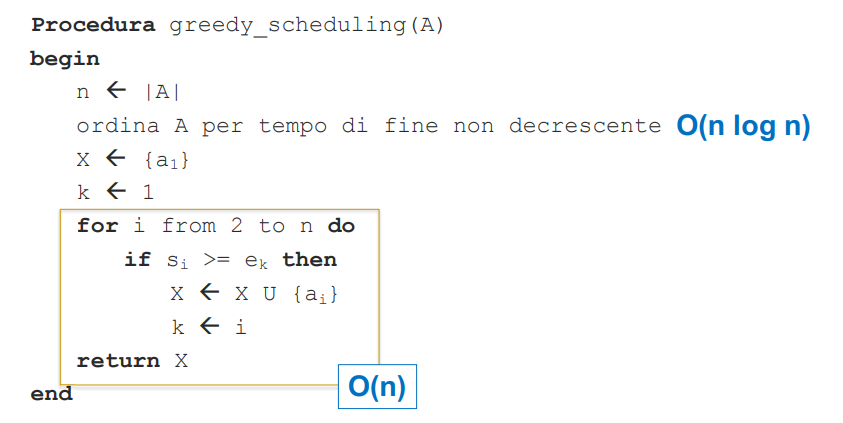
\includegraphics[width=80mm,scale=0.5]{greedy_code_ordinamento.png}
\end{center}
\section{Greedy VS DP}
\begin{itemize}
    \item Soluzione ottima \textbf{VS} Valore ottimo + Soluzione ottima
    \item Top-down \textbf{VS} Bottom-up
    \item Pochi sottoproblemi da risolvere \textbf{VS} Tanti sottoproblemi da risolvere
    \item Efficiente e semplice da scrivere \textbf{VS} Meno efficiente e più complicato da scrivere
    \item Applicabilità inferiore (te pareva) \textbf{VS} Applicabilità maggiore
\end{itemize}
\subsection{Due ingredienti chiave di un algoritmo Greedy}
\begin{itemize}
    \item Proprietà della sottostruttura ottima (tipica anche della Programmazione Dinamica)
    \item Proprietà della \textbf{scelta greedy}
\end{itemize}
Per la \textbf{Correttezza di un algoritmo Greedy} si deve DIMOSTRARE che la sequenza di scelte
localmente ottima conduce a una soluzione globalmente ottima.\\
\paragraph*{Proprietà della scelta greedy:} la scelta che compio ad ogni passo appartiene a una soluzione
ottima del sottoproblema che sto risolvendo in quel momento.
\section{Correttezza di un algoritmo Greedy}
Analizziamo la sottostruttura del problema della selezione di attività.
\paragraph*{Sottoproblema al passo generico:} Trovare il sottoinsieme di cardinalità massima di
attività compatibili, per l'insieme di attività che iniziano dopo la fine dell'attività aggiunta al passo
precedente.\\
\textbf{Sottoproblema 1}: sottoinsieme di cardinalità massima di attività compatibili,
per l'insieme A\\
\textbf{Sottoproblema 2}: sottoinsieme di cardinalità massima di attività compatibili, per 
l'insieme $A_2$ delle attività che hanno tempo di inizio $\geq$ al tempo di fine della
scelta fatta al passo 1.\\
...\\
\textbf{Sottoproblema k}: sottoinsieme di cardinalità massima di attività compatibili,
per l'insieme $A_k$ delle attività che hanno tempo di inizio $\geq$ al tempo di fine della
scelta fatta al passo $k-1$.\\
Scelta localmente ottima per il sottoproblema k \ra Attività $a_s$ con il minor tempo di fine
$A_k$.
\paragraph*{Proprietà della scelta greedy da dimostrare}
Ad ogni passo l'attività scelta è inclusa in una soluzione ottima del sottoproblema che sto risolvendo.
Basta dimostrare che \textbf{$a_1$ è inclusa in una soluzione ottima per l'insieme A}.\\
\subsection*{Dimostrazione}
Suppongo X soluzione ottima per A. Suppongo $a'_1$ attività con il minore tempo di fine X.\\
Se $a'_1$ uguale ad $a_1$ la dimostrazione è finita, altrimenti sostituisco in X l'attività
$a'_1$ con $a_1$.\\
Le attività in X sono ancora disgiunte. La dimensione di X non è cambiata.\\
\textbf{Conclusione:} il nuovo X è un sottoinsieme massimo di attività compatibili di A che include
ora $a_1$. 
\subsection{Cosa succede se sbaglio parametro?}
Consideriamo per esempio la durata massima come parametro, cosa succede alle soluzioni?\\
Prendendo l'esempio precedente notiamo subito che gli eventi della soluzione sarebbero i più
lunghi quindi $a_3$ e $a_6$ e questa non è una soluzione ottima.\\
Se scegliamo la durata minima otteniamo che in ordine di scelta $a_7,\, a_4,\, a_8$,
anche in questo caso questa non è una soluzione ottima.\\
Ci accorgiamo inoltre che i valori scelti inizialmente non sono soluzione ottima del sottoproblema,
mi rendo conto abbastanza velocemente quindi che sto sbagliando, ma analizziamo nel dettaglio
la questione considerando il seguente problema. 
\section{Il problema dello Zaino Frazionario}
Dati n oggetti $\langle 1,2,\dots,n \rangle$, un intero C e due funzoni.
\begin{itemize}
    \item $V:X \rt N$   $V(i) = v_i$, valore dell'oggetto i
    \item $W:X \rt N$   $W(i) = w_i$, peso dell'oggetto i
\end{itemize}
Trovare una sequenza $P = \langle p_1, p_2, \dots, p_n \rangle$ con $p_i$ in $[0,1]$ per
$1 \leq i \leq n$, tale per cui:
\[ \sum^n_{i=1}p_i w_i \leq C \]
\[ \sum^n_{i=1}p_i v_i \rt \text{ massimo valore} \]
In questo caso, a differenza del problema dello zaino 0/1, posso scegliere di frazionare gli oggetti,
quindi non devo per forza prendere tutto l'oggetto, ma posso prenderne anche solo una parte.
\section{Possibile strategia Greedy}
\begin{itemize}
    \item Ordino gli oggetti per valore non crescente
    \item Prendo la maggiore quantità del primo oggetto compatibile con la capacità dello zaino
    \item Prendo la maggiore quantità del secondo oggetto compatibile con la capacità residua dello zaino
    \item Prendo la maggiore quantità del terzo oggetto compatibile con la capacità residua dello zaino
    \item etc.
    \item Mi fermo non appena lo zaino è completamente pieno
\end{itemize}
Vediamo se questa strategia funziona:
\paragraph*{Istanza Problema}
Oggetti \ra $\langle 1,2,3 \rangle$
\begin{enumerate}
    \item $v_1 = 10$, $w_1 = 20$
    \item $v_2 = 9$, $w_2 = 8$
    \item $v_3 = 8$, $w_3 = 5$
\end{enumerate}
La capacità totale $C = 20$, mentre $c$ è la capacità residua.\\
Proviamo inserendo quindi la maggiore quantità di oggetto con valore maggiore.\\
Inserisco quindi l'oggetto 1, avendo capacità 20 e peso 20 posso inserirlo tutto.\\
Avendo peso 20 ho saturato completamente la capacità dello zaino e ho un valore di 10,
ottengo quindi che la soluzione $P = \langle 1,0,0 \rangle$ con appunto Valore \ra 10.\\
\'E facile osservare che NON si tratta della soluzione ottima, questo significa che ho sbagliato
a scegliere il parametro per la strategia Greedy.
\subsection{Cambio parametro}
Se scegliessi iniziassi a riempire lo zaino considerando il rapporto tra peso e valore, otterrei
i seguenti valori:
\begin{enumerate}
    \item $v_1 = 10$, $w_1 = 20, \frac{v_1}{w_1} = 0.5$
    \item $v_2 = 9$, $w_2 = 8, \frac{v_2}{w_2} = 1.125$
    \item $v_3 = 8$, $w_3 = 5, \frac{v_3}{w_3} = 1.6$
\end{enumerate}
Risulta quindi evidente che conviene inserire prima l'oggetto 3 perchè posso inserire
più parti di oggetto e avere più valori rispetto a inserire lo stesso peso degli altri.\\
Inserisco quindi tutto il terzo oggetto, occupando capacità 5, inserisco quindi il secondo oggetto,
che ha rapporto peso valore maggiore rispetto al primo. Dopo aver inserito il secondo oggetto,
noto di avere ancora dello spazio disponibile, quindi procedo a inserire il primo oggetto che però
non è possibile inserire tutto, ne inserisco quindi peso 7, cioè la capacità residua.\\
Ottengo quindi $P = \langle 0.35, 1, 1 \rangle$ e Valore \ra 20.5 che oltre a essere un valore
maggiore del primo tentativo è soluzione ottima. Questo è quindi il parametro corretto.
\subsection{Strategia Greedy Attuata}
\begin{itemize}
    \item Calcolo per ogni oggetto i il valore specifico $v_i/w_i$
    \item Ordino gli oggetti per valore specifico non crescente
    \item Prendo la maggiore quantità del primo oggetto compatibile con la capacità
    dello zaino
    \item Prendo la maggiore quantità del secondo oggetto compatibile con la capacità
    residua dello zaino
    \item ...
    \item Mi fermo appena lo zaino è completamente pieno
\end{itemize}
\paragraph*{Generico passo i} Scelta localmente ottima \ra percentuale di oggetto
i-esimo da prendere $p_i = min(c/w_i,1)$.\\
c è C diminuita del peso totale degli oggetti da 1 a i-1.\\
Sottoproblema lasciato dalla scelta di $p_i$:
\begin{itemize}
    \item Oggetti da i+1 a n
    \item Capacità C diminuita del peso totale degli oggetti da 1 a i
\end{itemize}
\subsection{Codice}
Inserire Codice
% Manca Codice
\subsection{Proprietà della scelta Greedy (da dimostrare)}
La percentuale $p_i$ scelta per l'oggetto i è inclusa in una soluzione ottima relativa al
sottoproblema:
\begin{itemize}
    \item oggetti da i a n
    \item Capacità residua dello zaino pari a C diminuita del peso totale degli
    oggetti aggiunti da 1 a i-1
\end{itemize}
Basta dimostrare la proprietà per la percentuale $p_1$ e sottoproblema:
\begin{itemize}
    \item Oggetti da 1 a n
    \item Capacità C dello zaino
\end{itemize}
\section{Algoritmi Greedy in Generale}
\subsection{Codice generico}
\begin{lstlisting}[language=Java, escapeinside={@*}{*@}]
    Procedura general_greedy(S = {@*$s_1,s_2,...,s_n$*@})
        Calcola per ogni elemento un certo parametro
        Ordina S sulla base del parametro calcolato
        X = @*$\emptyset$*@
        for i from 1 to n do
            if @*$s_i$*@ is la scelta localmente ottima then
                X = @*$\{s_i\} \cup X$*@
        return X
\end{lstlisting}
\section{Non tutti i problemi ammettono un algoritmi Greedy}
Il problema zaino 0/1 non ammette un algoritmo di tipo greedy come soluzione.
Nelle slide vengono fatti degli esempi che mostrano che è impoddibile identificare
una strategia greedy valida.\\
Questo perchè non tutti i problemi ammettono un algoritmo Greedy, ma la vera questione
è: \textbf{Come capire, in linea di principio, se un problema ammette un algoritmo Greedy?}.\\
Per capire questo aspetto dobbiamo introdurre una struttura denominata Matroide.
\paragraph*{Matroide:} struttura combinatoria a cui è associato un algoritmo greedy.
\subsection{Sistema di Indipendenza}
Una coppia (S,F)
\begin{itemize}
    \item S, insieme finito $\{s_1, s_2, \dots, s_n\}$ di elementi
    \item F, una famiglia di sottoinsiemi di S, cioè un sottoinsieme dell'insieme P(S)
    delle parti di S
\end{itemize}
\paragraph*{Esempio} 
\begin{align*}
    &S = \{1,2,3\}\\
    &P(S) = \{\emptyset, \{1\},\{2\},\{3\},\{1,2\},\{1,3\},\{2,3\},\{1,2,3\}\}\\
    &F=\{\{1\},\{3\},\{1,3\}\}\\
\end{align*}
Una coppia (S,F) così definita è un \textbf{Sistema di Indipendenza} se vale la seguente
proprietà:\\
\textbf{preso $A \in F$ allora un qualsiasi $B \subseteq A$ appartiene a F}.\\
Elementi di F \ra sottoinsiemi indipendenti.\\
\paragraph*{Esempio}
\begin{itemize}
    \item S, insieme $\{1,2,...,n\}$ di n oggetti a cui è associato un peso
    \item F, famiglia dei sottoinsiemi di S che hanno peso totale $\leq$ C
\end{itemize}
è un Sistema di Indipendenza, cioè:\\
$A \in F, \, B \subseteq A \implies B \in F$\\
\paragraph*{PROOF:} Se $A \in F$, allora il suo peso totale è $\leq$ C.\\
Un qualsiasi $B \subseteq A$, avrà peso totale $\leq$ C e quindi anche $B \in F$.\\
\subsection{Proprietà di scambio}
Un sistema di Indipendenza (S,F) è un \textbf{matroide} se vale la seguente
\textbf{proprietà di scambio}:\\
\textbf{Per qualsiasi A, $B \in F$ tali che $|B|=|A|+1$, allora esiste almeno un elemento
$b \in B-A$ tale che $\{b\}\cup A \in F $}.\\
\paragraph*{NB} in un matroide l'insieme vuoto è un insieme indipendente.
\paragraph*{Esempio 1} Coppia (S,F):
\begin{itemize}
    \item S, insieme finito di oggetti
    \item F, famiglia dei sottoinsiemi di S di cardinalità $\leq k$
\end{itemize}
(S,F) è un Sistema di Indipendenza, cioè:\\
$A \in F, \, B \subseteq A \implies B \in F$\\
\textbf{PROOF}: Se $A \in F$, allora la sua cardinalità è $\leq k$.\\
Un qualsiasi $B \subseteq A$ avrà cardinalità $\leq k$ e quindi anche $B \in F$.
